\section{Aprendizado de máquina}

Aprendizado pode ser definido como qualquer mudança em um sistema que
otimize o seu desempenho na segunda vez que ele repetir a mesma tarefa,
ou outra tarefa da mesma população~\cite{custodio2010aprendizadomaquina}.

O aprendizado de máquina utiliza um princípio de inferência denominado
indução, onde através de um conjunto particular de exemplos é possível
obter conclusões genéricas~\cite{bruno2010aprendizadomaquina}. De um modo
abstrato o aprendizado de máquina funciona como uma caixa preta, onde
independente de como é implementado, o mesmo deve ser capaz de encontrar padrões
nos dados apresentados e criar um modelo para dados que ainda não foram vistos.

Como exemplo, o aprendizado de máquina pode ser usado para classifcar
um conjunto de atributos. Exemplo assim são bastante comuns quando se fala em
aprendizado de máquina. \citeonline{lecun1989backpropagation} usou algoritmos de
aprendizado de máquina para classificar códigos postais escritos a mão. Outro
exemplo está no trabalho de \citeonline{stallkamp2012man}, que usa método de
aprendizado de máquina para classificar placas de trânsito em diferentes
condições.


\subsection{Aprendizado supervisionado}

Quando se fala de aprendizado de máquina, várias técnicas distintas podem ser
usadas, entretanto, uma das principais técnicas de aprendizado de máquina é o aprendizado
supervisionado, onde é fornecido um treinamento com o conhecimento do
ambiente, que é composto por um conjunto de exemplos com entradas
e uma saída esperada~\cite{bruno2010aprendizadomaquina}.

O objetivo do aprendizado supervisionado é induzir conceitos a partir de
exemplos que estão pré-classificados, em outras palavras, exemplos que
possuem um rótulo associado a uma classe conhecida~\cite{bruno2010aprendizadomaquina}.
Utilizado quando se tem tanto as perguntas quanto as respostas, o aprendizado
supervisionado é utilizado para se obter uma classificação e funções de aproximação, ou seja,
tais algoritmos produzem um modelo à partir de dados já classificados capaz de estimar classificações
para dados ainda não vistos.

Utilizando do exemplo do algoritmo que classifica um conjunto de atributos,
na utilização do aprendizado supervisionado, para cada entrada do treinamento
existe um rótulo, que se trata da classificação do conjunto de atributos, ou
seja, apenas possui os valores 0, 1 e 2, entrada também possui os valores dos
atributos associados ao rótulo. A tabela~\ref{tab:entradas_de_treinamento}
mostra um exemplo das entradas de treinamento.

\begin{table}[h]
\centering
\resizebox{\textwidth}{!}{\begin{tabular}{|l|l|l|l|l|l|}
\hline
\rowcolor[HTML]{EFEFEF}
{\textbf{Rótulo}} & {\textbf{Atributo 1}} & {\textbf{Atributo 2}} & {\textbf{Atributo 3}} & {\textbf{Atributo 4}} & {\textbf{Atributo 5}} \\ \hline
1 & 1 & 0 & 1 & 0 & 1 \\
\hline
2 & 0 & 1 & 1 & 0 & 1 \\
\hline
0 & 1 & 0 & 0 & 1 & 1 \\
\hline
1 & 1 & 0 & 1 & 1 & 0 \\
\hline
2 & 0 & 1 & 1 & 1 & 0 \\
\hline
\end{tabular}}
\caption{Entradas de treinamento para o aprendizado de máquina}
\label{tab:entradas_de_treinamento}
\end{table}

Após ser realizada a etapa de treinamento, ao receber uma sequencia de cinco
atributos, o algoritmo deve retornar qual o rótulo, ou seja, a classificação,
correspondente a esses atributos. A tabela~\ref{tab:entrada_para_classificar}
mostra um exemplo de entrada para o algoritmo, a diferença dessa entrada para
a de treinamento é que essa não possui o rótulo, pois o rótulo será o resultado
da execução do algoritmo.

\begin{table}[h]
\centering
\resizebox{\textwidth}{!}{\begin{tabular}{|l|l|l|l|l|}
\hline
\rowcolor[HTML]{EFEFEF}
{\textbf{Atributo 1}} & {\textbf{Atributo 2}} & {\textbf{Atributo 3}} & {\textbf{Atributo 4}} & {\textbf{Atributo 5}} \\ \hline
1 & 0 & 1 & 1 & 0 \\
\hline
\end{tabular}}
\caption{Entrada de dados para o algoritmo determinar o rótulo}
\label{tab:entrada_para_classificar}
\end{table}


\subsection{Classificador Bayesiano}

Uma técnica famosa de algoritmos supervisionados é o classificador bayesiano,
que é normalmente chamado de \textit{naive bayes}. Esse algoritmo é baseado no
princípio da probabilidade bayesiana, entretanto, diferente do modelo em si,
ele admite que os atributos de um dado são sempre independentes um do outro,
mesmo que os atributos possuam alguma dependência um do outro \cite{segaran2007programming}

Sendo assim, o classificador bayesiano irá basicamente classificar um dado
como pertencente a uma classe, se tal classe obter o maior valor de
probabilidade dentre os valores de classe possíveis. Dessa forma, pode-se
dizer que a classificação bayesiana segue o seguinte formato:

$Classificador = max(p(C_{y})*\prod_{i=1}^{N}p(x_{i}|C_{y}))$

Onde:

\begin{itemize}
    \item \textbf{$C_{y}$: } Uma das classes possíveis para classificar um
    dado;
    \item \textbf{n: } Número total de itens;
    \item \textbf{$p(C_{y})$: } Probabilidade da classe ``y'' dentro do
    conjunto de dados. Pode ser calculado pela
    fórmula: $\frac{NC_{y}}{N_{t}}$.
    Onde:
      \begin{itemize}
          \item \textbf{$NC_{y}$: } Número de itens da classe ''y'';
          \item \textbf{$N_{t}$: } Número total de classes;
      \end{itemize}
    \item \textbf{$p(x_{i}|C_{y})$: } Cálculo da probabilidade bayesiana
    em si, assumindo que as variáveis são independentes. Tal expressão
    pode ser calculada pela seguinte fórmula: $\frac{Nxi_{C_{y}}}{NC_{y}}$.
    Onde $Nxi_{C_{y}}$ é o número de vezes que o atributo $x_{i}$ aparece
    dentro de um dado marcado como $C_{y}$.
\end{itemize}

Dessa forma, pode-se ver o modelo gerado por esse algoritmo supervisionado
é nada mais com que as probabilidades $p(C_{y})$ e $p(x_{i}|C_{y})$ para
todas as possíveis classificações que serão usadas no problema. Dessa forma,
os dados usados para alimentar tal algoritmo são para criar exatamente tais
dados. Uma vez com eles calculados, o modelo do algoritmo está completo,
podendo o mesmo ser usado para classificar dados ainda não vistos.

Vale ressaltar que o modelo apresentado tem como base a classificação
bayesiana usando o modelo de Bernoulli, onde os valores de $x_{i}$ são valores
binários, indicando assim a presença ou não de um atributo em um certo dado.
Para valores discretos, pode-se usar outros modelos, como o Gaussiano, onde
seria necessário o cálculo da média e variância dos atributos para as dadas
classes de classificação \cite{zhang2004optimality}.

Apesar da simplicidade desse algoritmo, alguns cuidados devem ser observados.
O primeiro cuidado é analisar as variáveis, pois quando estas possuem uma grande
dependência entre elas, pode levar o modelo a acarretar problemas. O outro cuidado
se dá no uso dos atributos que são usados para gerar a classificação de um dado.
Apesar dessa preocupação estar presente em algoritmos supervisionados em geral,
o número de cálculos necessários para esse sistema aumenta consideravelmente a
cada novo atributo adicionado, podendo assim ocasionar problemas de performance.

\subsection{Engenharia de atributos}

Considerando que aprendizado de máquina tem como um alicerce os dados de entrada
e principalmente as características desses dados, deve-se ter um cuidade
significativo em selecionar os atributos que serão usados para alimentar um
algoritmo de aprendizado de máquina. Essa problemática se torna ainda maior
quando um dado apresentado possui um conjunto de atributos muito grande, ou
seja, possui uma dimensao alta. Quando isso acontece, pode-se dizer que a
densidade entre os dados e as distâncias entre os mesmos se tornam menos
significativas \cite{amatriain2011data}. Esse efeito se chama \textit{maldição
da dimensionalidade} e pode afetar negativamente um série de algoritmos de
aprendizado de máquina.

Um dos efeitos diretos desse problema é o caso chamado de \textit{overfitting}.
Esse problema acontece quando um algoritmo fica viciado nas entradas em qual foi
treinado e não apresenta resultados satisfatórios quando recebe dados que nunca
viu. Sendo assim, uma das formas de evitar tal problema é selecionar bem os
atributos de um projeto ou até mesmo usar técnicas para diminuir a
dimensionalidade de uma variável de entrada.

Caso a seleção seja manual, é recomendável que a mesma seja realizada ao lado de
um especialista na área na qual o aprendizado de máquina será utilizado. Isso se
dá pela capacidade de um profissional da área em informar que atributos são
relevantes para a classicação de um determindado objeto.

O segundo método se dá pelo uso de técnicas computacionais para reduzir a
dimensão de uma variável. Um exemplo dessa técnica é o \textit{Principal
Component Analysis (PCA) } que ordena os atributos que maior contribuem para a
variância dos dados em relação ao método de mínimos quadrados
\cite{amatriain2011data}. Normalmente, tal método ignora atributos após a
variãncia acumulada passar de 90\%.

Apesar da aplicação de ambas as formas em conjunto serem possíveis, vale lembrar
que ambas possuem limitações. Para a seleção manual de atributos, pode-se ter
casos onde a classificação dos dados nunca foi feita ou até mesmo a dificuldade
em se encontrar um especialista na área para ajudar na seleção. Enquanto isso,
para algoritmos de redução, algumas limitações também existem. Para o caso do
PCA, o mesmo parte do pressuposto que os dados apresentados seguem uma
distribuição Gaussiana. Quando isso não acorre, nada pode-se garantir quanto a
seleção dos atributos mais significativos \cite{amatriain2011data}. Mesmo com
essas dificuldades, essa etapa é crucial para um bom funcionamento do algoritmo
de aprendizado de máquina, principalmente quanto a escalabilidade do mesmo.


\subsection{Validação cruzada}

Uma das formas de validar se o algoritmo não está sofrendo \textit{overfitting}
e o seu oposto, \textit{undefitting}, onde o algoritmo apresenta elevado valor
de \textit{bias} para as entradas usadas como teste, ou seja, o modelo criado
pelo algoritmo é muito simples. Uma forma de observar a ocorrência desses dois
fenômenos é pela técnica estatística de validação cruzada. Essa técnica é
comumente usada para avaliar modelos preditivos, e se baseia na separação dos
dados existentes em uma parte de treinamento e uma parte de teste. A conjunto de
dados de treinamento é usado para alimentar o algoritmo. Após o treinamento,
e o conjunto de teste é então usado para validar o algoritmo. \cite{araujo2011apprecommender}.

Uma forma de tornar o processo de validação cruzada visual é o uso de curvas de
aprendizado. Uma curva de aprendizado pode ser vista como a relação das curvas
erro do conjunto de dados de treinamento e a curva dos dados de teste. Isso pode
ser visto como melhor foco na Figura \ref{fig:curva_aprendizado}.

\begin{figure}[h]
  \centering
  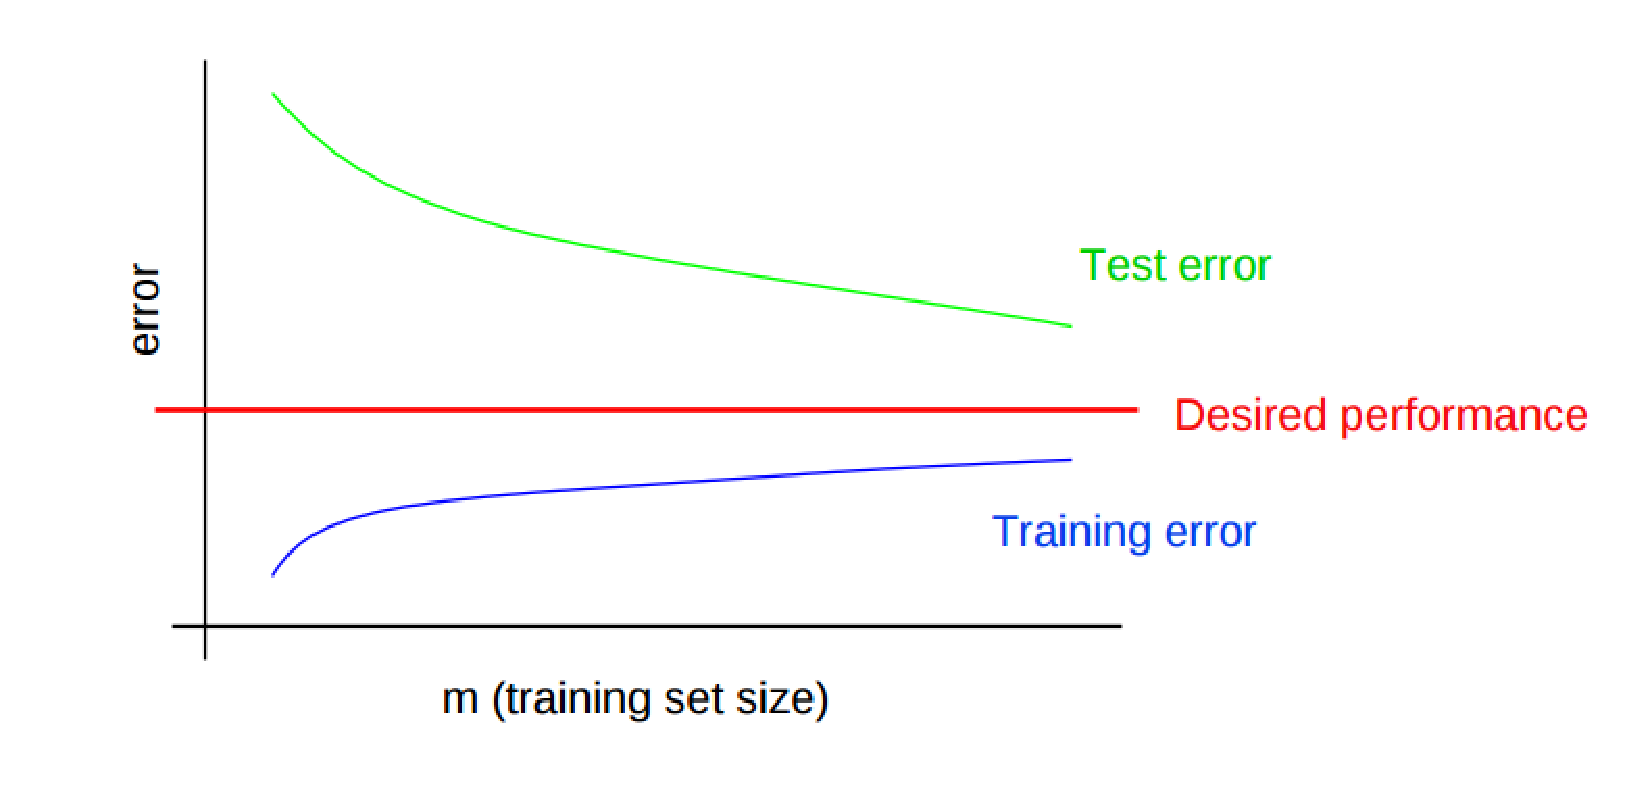
\includegraphics[width=0.9\textwidth]{figuras/curva_aprendizado.eps}
  \caption{Exemplo de uma curva de aprendizado \cite{1_ng} }
  \label{fig:curva_aprendizado}
\end{figure}

Pode-se ver na figura \ref{fig:curva_aprendizado}, o eixo das ordenadas representa o valor do erro, enquanto
o erro das abscissas representa o tamanho do conjunto de dado usado para treinamento. Para calcular
o erro apresentado nos gráficos, pode-se usar qualquer fórmula estatística para tal fim. Entretanto, uma das mais comuns
quando se trata de validação cruzada é a seguinte \cite{1_ng}:

\begin{equation}
ErroTreinamento = \frac{1}{2m}*\sum_{i=0}^{m}(h(x_{i}) - y(x_{i}))^2
\end{equation}

\begin{equation}
ErroTeste = \frac{1}{2m_{teste}}*\sum_{i=0}^{m_{teste}}(h(x_{t}^{i}) - y(x_{t}^{i}))^2
\end{equation}

Onde:

\begin{itemize}
    \item \textbf{m: } Tamanho do conjunto de teste;
    \item \textbf{$h(x_{i}$): } Função que reflete o modelo criado por um algoritmo de aprendizado de máquina, ou seja, recebe um dado e retorna um classificação.
    \item \textbf{$y(x): $} Valore real da classificação para o dado sendo apresentado
    \item \textbf{$m_{teste}$: } Tamanho do conjunto de teste obtido por validação cruzada.
\end{itemize}

Dessa forma, pode-se ver que o gráfico mostra a evolução do modelo produzido pelos dados de treinamento
em relação ao conjunto de dados obtidos pela validação cruzada, variando-se o número de dados usados no treinamento. É esperado que inicialmente, as curvas fiquem bem distantes
uma da outra, pois com poucos dados de treinamento, o conjunto de teste apresentára erros altos, enquanto o conjunto de treinamento não. Entrentanto, com mais dados de treinamento
usados, é esperado que as curvas se aproximem mais uma da outra.

O uso desses gráficos pode-se bastante útil para encontrar casos de \textit{overfitting} e \textit{underfitting} pois tais casos podem ser claramente identificados
observando-se o gráfico. Em um conjunto de teste onde ao final, as curvas de treinamento erro estão muito distantes, pode-se entender que o algoritmo
está apresentando \textit{underfitting}. Entretanto, caso as curvas estejam muito próximas quando se usa todos os dados de treinamento alocados, pode-se entender
uma baixa variância do modelo, identificando assim um caso de \textit{overfitting}.

\subsection{Bayes Ingênuo}

Um algoritmo supervisionado, e bastante utilizado no aprendizado de máquina,
o bayes ingênuo, também conhecido como naive bayes, é denominado ingênuo devido
ao fato de que o algoritmo assume que os atributos são condicionalmente
independentes, ou seja, considera-se que as entradas são independentes entre
si, porém, mesmo partindo dessa ingenuidade os resultados não comprometem a
qualidade~\cite{bruno2010aprendizadomaquina}. Mesmo com essa independencia dos
atributos, o bayes ingênuo é um método bastante efetivo e frequentemente oferece
uma precisão comparável aos outros métodos (comparável à métodos pertencentes ao
estado da arte), e estudos também mostram que o bayes ingênuo pode aprender a
função de classificação ótima~\cite{santos2010naivebayes}.

No caso da classificação dos atributos, onde para cada entrada há o rótulo, ou
seja, a classificação, seguido dos cinco atributos que possuem essa classificação,
como mostra a tabela~\ref{tab:entradas_de_treinamento}. Na utilização do Bayes
Ingênuo a tabela~\ref{tab:entradas_de_treinamento} será dividida em uma matriz D
com os dados dos atributos, as dimensões dessa matriz são ``${e \times a}$'', onde
``e'' é o número de entradas e ``a'' é o número de atributos, e a outra parte da
divisão da tabela~\ref{tab:entradas_de_treinamento} é um vetor coluna L com os
dados dos rótulos, onde suas dimensões são ``${e \times 1}$''.

$$D=\left[
\begin{array}{ccccc}
1 & 0 & 1 & 0 & 1 \\
0 & 1 & 1 & 0 & 1 \\
1 & 0 & 0 & 1 & 1 \\
1 & 0 & 1 & 1 & 0 \\
0 & 1 & 1 & 1 & 0 \\
\end{array}
\right]_{e \times a}$$

$$L=\left[
\begin{array}{c}
1 \\
2 \\
0 \\
1 \\
2 \\
\end{array}
\right]_{e \times 1}$$

Para o algoritmo funcionar também é necessário ter conhecimento de quais são as
classificações que os atributos podem receber, essas classificações são informadas
através do vetor coluna B, com dimensões ``${l \times 1}$'', onde ``l'' é o número
de rótulos, ou classificações possíveis.

$$B=\left[
\begin{array}{c}
0 \\
1 \\
2 \\
\end{array}
\right]_{l \times 1}$$

Utilizando a matriz D e os vetores L e B, monta-se a matriz de adjacência A, onde
cada linha dessa matriz representa respectivamente uma linha do vetor B, e cada
coluna da matriz representa um atributo. A matriz de adjacência A também é uma
matriz com valores binários, onde um indica a presença do atributo na classificação,
e zero indica a ausência do atributo na classificação. Logo a matriz A possui
dimensões ``${l \times e}$''.

$$A=\left[
\begin{array}{ccccc}
0 & 0 & 1 & 0 & 0 \\
1 & 0 & 0 & 1 & 0 \\
0 & 1 & 0 & 0 & 1 \\
\end{array}
\right]_{e \times a}$$

Utilizando a matriz A pode-se calcular o vetor com o histograma do vetor L, onde
cada linha do vetor histograma H representa respectivamente um possível rótulo da
matriz B, e o valor de cada linha representa o número de pacotes no qual o rótulo
está associado. O vetor coluna H é calculado pela multiplicação da matriz A pelo
vetor coluna com todos os valores sendo 1, onde esse vetor coluna possui ``e''
linhas, logo as dimensões do vetor coluna H são ``${l \times 1}$''

$$H=A * \left[
\begin{array}{c}
1 \\
1 \\
1 \\
1 \\
1 \\
\end{array}
\right]_{e \times 1}$$

$$H=\left[
\begin{array}{c}
1 \\
2 \\
2 \\
\end{array}
\right]_{l \times 1}$$

Utilizando o vetor H é calculado a probabilidade de cada rótulo, que é representada
pelo vetor PH, resultante da divisão do vetor H por ``e''.

\begin{center}
$PH= \frac{1}{e} * H$
\end{center}

$$PH=\left[
\begin{array}{c}
\frac{1}{3} \\
\frac{2}{3} \\
\frac{2}{3} \\
\end{array}
\right]_{l \times 1}$$

O próximo passo é calcular a matriz PR1, que se trata da probabilidade de um
atributo ser igual a um, na relação entre os rótulos possíveis, o vetor B, e os
atributos da matriz D. Para isso é necessário identificar quantos atributos cada
rótulo possui, obtido pela multiplicação da matriz de adjacência A com a matriz
de dos atribudos D, resultando na matriz R contendo para cada possível rótulo
quantos atributos este possui. A matrix PR1 é resultado da multiplicação entre a
matriz inversa da diagonal feita pelo vetor H com a matriz R.

\begin{center}
$R = A * D$
\end{center}

$$R=\left[
\begin{array}{ccccc}
1 & 0 & 0 & 1 & 1 \\
2 & 0 & 2 & 1 & 1 \\
0 & 2 & 2 & 1 & 1 \\
\end{array}
\right]_{l \times a}$$

$$diag(H)=\left[
\begin{array}{ccc}
\frac{1}{3} & 0 & 0 \\
0 & \frac{2}{3} & 0 \\
0 & 0 & \frac{2}{3} \\
\end{array}
\right]_{l \times l}$$

$$diag(H)^{-1}=\left[
\begin{array}{ccc}
1 & 0 & 0 \\
0 & \frac{1}{2} & 0 \\
0 & 0 & \frac{1}{2} \\
\end{array}
\right]_{l \times l}$$

\begin{center}
$PR1 = diag(H)^{-1} * R$
\end{center}

$$PR1=\left[
\begin{array}{ccccc}
1 & 0 & 0 & 1 & 1 \\
1 & 0 & 1 & \frac{1}{2} & \frac{1}{2} \\
0 & 1 & 1 & \frac{1}{2} & \frac{1}{2} \\
\end{array}
\right]_{l \times a}$$

Também é necessário identificar a matriz PR0, que indica a probabilidade dos
atributos possuirem o valor zero, essa matriz pode ser obtida através da
expressão ``$1 - PR1$''.

\begin{center}
$PR0 \ = \ 1 \ - \ PR1$
\end{center}

$$PR0=\left[
\begin{array}{ccccc}
0 & 1 & 1 & 0 & 0 \\
0 & 1 & 0 & \frac{1}{2} & \frac{1}{2} \\
1 & 0 & 0 & \frac{1}{2} & \frac{1}{2} \\
\end{array}
\right]_{l \times a}$$

É necessário transformar as matrizes PR1 e PR0 em matrizes quadradas,
sendo suas dimensoes ``${l \times a}$'', a matriz quadrada deve possuir
a maior dentre as duas dimensões, neste caso as matrizes devem possuir
as dimensões ``${a \times a}$'', para que isso aconteça as matrizes são
multiplicadas pela matriz identidade de dimensões ``${a \times l}$''.

$$PR1=\left[
\begin{array}{ccc}
1 & 0 & 0 \\
0 & 1 & 0 \\
0 & 0 & 1 \\
0 & 0 & 0 \\
0 & 0 & 0 \\
\end{array}
\right]_{a \times l}
\left[
\begin{array}{ccccc}
1 & 0 & 0 & 1 & 1 \\
1 & 0 & 1 & \frac{1}{2} & \frac{1}{2} \\
0 & 1 & 1 & \frac{1}{2} & \frac{1}{2} \\
\end{array}
\right]_{l \times a}
= \left[
\begin{array}{ccccc}
1 & 0 & 0 & 1 & 1 \\
1 & 0 & 1 & \frac{1}{2} & \frac{1}{2} \\
0 & 1 & 1 & \frac{1}{2} & \frac{1}{2} \\
0 & 0 & 0 & 0 & 0 \\
0 & 0 & 0 & 0 & 0 \\
\end{array}
\right]_{a \times a}$$

$$PR0=\left[
\begin{array}{ccc}
1 & 0 & 0 \\
0 & 1 & 0 \\
0 & 0 & 1 \\
0 & 0 & 0 \\
0 & 0 & 0 \\
\end{array}
\right]_{a \times l}
\left[
\begin{array}{ccccc}
0 & 1 & 1 & 0 & 0 \\
0 & 1 & 0 & \frac{1}{2} & \frac{1}{2} \\
1 & 0 & 0 & \frac{1}{2} & \frac{1}{2} \\
\end{array}
\right]_{l \times a}
= \left[
\begin{array}{ccccc}
0 & 1 & 1 & 0 & 0 \\
0 & 1 & 0 & \frac{1}{2} & \frac{1}{2} \\
1 & 0 & 0 & \frac{1}{2} & \frac{1}{2} \\
0 & 0 & 0 & 0 & 0 \\
0 & 0 & 0 & 0 & 0 \\
\end{array}
\right]_{a \times a}$$

Obtendo o vetor PH, que é a probabilidade individual de cada rótulo, e a
matrizes PR1 e PR0, que são a probabilidade da relação entre os rótulos
possíveis e os atributos da matriz D, o treinamento do algoritmo está
finalizado.

Com o algoritmo treinado, ele está pronto para receber um vetor com
os atributos, como mostra a tabela~\ref{tab:entrada_para_classificar},
é usado como exemplo o vetor v, que possui dimensões ``${1 \times a}$''.

$$v=\left[
\begin{array}{ccccc}
1 & 0 & 1 & 1 & 0 \\
\end{array}
\right]_{1 \times a}$$

O próximo passo é montar a matriz PV, que se trata da matriz de
probabilidade para o vetor, onde se trata da junção das matrizes
PR1 e PR0, onde para cada coluna do vetor v, se o valor for um
utiliza a coluna da matriz PR1, se o valor for zero, utiliza a
coluna da matriz PR0. Em outras palavras, a matriz PV é resultante
da soma dos produtos entre PR1 e a matriz diagonal de v, com PR0
e a matriz diagonal de v', onde o vetor v' se trata do vetor v
porém os valores de 1 e 0 são alternados.

$$v'=1-\left[
\begin{array}{ccccc}
1 & 0 & 1 & 1 & 0 \\
\end{array}
\right]_{1 \times a}
=
\left[
\begin{array}{ccccc}
0 & 1 & 0 & 0 & 1 \\
\end{array}
\right]_{1 \times a}
$$
\\

\begin{center}
$PV = PR1 * diagonal(v) \ + \ PR0 * diagonal(v')$
\end{center}

$$PV=
\left[
\begin{array}{ccccc}
1 & 0 & 0 & 1 & 1 \\
1 & 0 & 1 & \frac{1}{2} & \frac{1}{2} \\
0 & 1 & 1 & \frac{1}{2} & \frac{1}{2} \\
0 & 0 & 0 & 0 & 0 \\
0 & 0 & 0 & 0 & 0 \\
\end{array}
\right]_{a \times a}
\left[
\begin{array}{ccccc}
1 & 0 & 0 & 0 & 0 \\
0 & 0 & 0 & 0 & 0 \\
0 & 0 & 1 & 0 & 0 \\
0 & 0 & 0 & 1 & 0 \\
0 & 0 & 0 & 0 & 0 \\
\end{array}
\right]_{a \times a}
+
\left[
\begin{array}{ccccc}
0 & 1 & 1 & 0 & 0 \\
0 & 1 & 0 & \frac{1}{2} & \frac{1}{2} \\
1 & 0 & 0 & \frac{1}{2} & \frac{1}{2} \\
0 & 0 & 0 & 0 & 0 \\
0 & 0 & 0 & 0 & 0 \\
\end{array}
\right]_{a \times a}
\left[
\begin{array}{ccccc}
0 & 0 & 0 & 0 & 0 \\
0 & 1 & 0 & 0 & 0 \\
0 & 0 & 0 & 0 & 0 \\
0 & 0 & 0 & 0 & 0 \\
0 & 0 & 0 & 0 & 1 \\
\end{array}
\right]_{a \times a}
$$

$$PV=\left[
\begin{array}{ccccc}
1 & 1 & 0 & 1 & 0 \\
1 & 1 & 1 & \frac{1}{2} & \frac{1}{2} \\
0 & 0 & 1 & \frac{1}{2} & \frac{1}{2} \\
0 & 0 & 0 & 0 & 0 \\
0 & 0 & 0 & 0 & 0 \\
\end{array}
\right]_{a \times a}$$

Através da matriz PV é obtido o vetor coluna ``u'', onde o cada linha
do vetor u corresponde a multiplicação dos elementos da linha da matriz
PV, porém devido ao fato de uma probabilidade zero em uma linha da matriz
PV irá fazer com que a multiplicação da linha seja igual a zero, para
impedir esse problema é somado 1 a matriz PV. Como a matriz pode ter
centenas de atributos ``a'' existe o problema de que a multiplicação
desses elementos tornem a multiplicação das linhas da matriz um número
muito grande, ou um número muito pequeno, afim de impedir que ocorra
problemas computacionais com o tamanho dos números, ao invés de multiplicar
as linhas da matriz, é somado o log de cada elemento da matriz PV resultando
no vetor ``u''.

\begin{center}
$PV = PV + 1$
$$PV=\left[
\begin{array}{ccccc}
2 & 2 & 1 & 2 & 1 \\
2 & 2 & 2 & \frac{3}{2} & \frac{3}{2} \\
1 & 1 & 2 & \frac{3}{2} & \frac{3}{2} \\
1 & 1 & 1 & 1 & 1 \\
1 & 1 & 1 & 1 & 1 \\
\end{array}
\right]_{a \times a}$$
\end{center}

\begin{center}
$PV = log(PV)$
$$PV=\left[
\begin{array}{ccccc}
0.69315 & 0.69315 & 0.00000 & 0.69315 & 0.00000 \\
0.69315 & 0.69315 & 0.69315 & 0.40547 & 0.40547 \\
0.00000 & 0.00000 & 0.69315 & 0.40547 & 0.40547 \\
0.00000 & 0.00000 & 0.00000 & 0.00000 & 0.00000 \\
0.00000 & 0.00000 & 0.00000 & 0.00000 & 0.00000 \\
\end{array}
\right]_{a \times a}$$
\end{center}

\begin{center}
$u \ = \ soma Das Linhas de PV$
$$u=\left[
\begin{array}{c}
2.07944 \\
2.89037 \\
1.50408 \\
0.00000 \\
0.00000 \\
\end{array}
\right]_{a \times 1}$$
\end{center}

Assim como foi feita uma operação nas matrizes PR1 e PR0 para que as
matrizes fiquem quadradas, é necessário que o vetor u tenha a mesma
dimensão do vetor B, que é o vetor com os os possíveis labels, para
isso multiplica-se o vetor u pela diagonal unitária com dimensão
quantidade de labels ``l'' pela quantidade de atributos ``a''.

$$u=\left[
\begin{array}{ccccc}
1 & 0 & 0 & 0 & 0 \\
0 & 1 & 0 & 0 & 0 \\
0 & 0 & 1 & 0 & 0 \\
\end{array}
\right]_{l \times a}
\left[
\begin{array}{c}
2.07944 \\
2.89037 \\
1.50408 \\
0.00000 \\
0.00000 \\
\end{array}
\right]_{a \times 1}
$$

$$u=\left[
\begin{array}{c}
2.07944 \\
2.89037 \\
1.50408 \\
\end{array}
\right]_{l \times 1}
$$

O vetor PF contendo a probabilidade de cada rótulo para o vetor de
entrada v, é obtido pela relação entre a probabilidade de cada rótulo,
o vetor PH, com o vetor u, onde PF é o resultado da multiplicação da
diagonal do vetor PH com o vetor u, onde o vetor PH deve passar pelo
mesmo processo do vetor PV, ou seja, somar 1 ao vetor e depois fazer
o log.

\begin{center}
$PH = 1 + PH$
$$PH=\left[
\begin{array}{c}
\frac{4}{3} \\
\frac{5}{3} \\
\frac{5}{3} \\
\end{array}
\right]_{l \times 1}$$
\end{center}

\begin{center}
$PH = log(PH)$
$$PH=\left[
\begin{array}{c}
0.28768 \\
0.51083 \\
0.51083 \\
\end{array}
\right]_{l \times 1}$$
\end{center}

$$PF=\left[
\begin{array}{ccccc}
0.28768 & 0 & 0 \\
0 & 0.51083 & 0 \\
0 & 0 & 0.51083 \\
\end{array}
\right]_{l \times l}
\left[
\begin{array}{c}
2.07944 \\
2.89037 \\
1.50408 \\
\end{array}
\right]_{l \times 1}
$$

$$PF=\left[
\begin{array}{c}
0.59822 \\
1.47648 \\
0.76832 \\
\end{array}
\right]_{l \times 1}
$$

O rótulo que possui maior probabilidade para o vetor de entrada v, é o
rótulo 1, ou a classificação 1 para o exemplo, pois o rótulo 1 no vetor
B está na mesma linha que a maior probabilidade no vetor PF. Logo a resposta
do algoritmo para a entrada do vetor v é o rótulo 1, essa é a aplicação
do algoritmo naive bayes para o exemplo da classificação do conjunto de
atributos.

O classificador bayesiano pode ser calculado através do modelo de probabilidade
máxima posterior, ``dado que C é o conjunto de classes e x o objeto a ser
classificado, a classe atribuída será a que apresentar maior probabilidade
condicionada a x. {\^P} é utilizado em vez de P porque geralmente não se sabe
o valor exato das probabilidades, que são estimadas a partir dos dados de
treinamento''\citeonline{araujo2011apprecommender}.

\begin{center}
$ c_{map} \ = \ {arg max}_{c \in C} \ \hat{P}(c) \ \prod\limits_{1 \leq i \leq n} \hat{P}(x_i | c)  $
\\
\end{center}

Onde {\^P}(c) se trata dos valores do vetor PH, o produtório $\hat{P}(x_i | c)$
é representado pelo vetor u, e a seleção do maior arguemento de ${c \in C}$
acontece na seleção do elemento do vetor B, que representa os rótulos que os
atributos podem receber, relacionado a mesma linha do maior elemento no vetor PF,
que representa a probabilidade associada a cada rótulo.
